\documentclass[12pt,a4paper]{article}
\usepackage{fontspec}
\setmainfont{Times New Roman}
\setsansfont{Arial}
\setmonofont{Courier New}
\usepackage[provide=*,english,romanian]{babel}
\usepackage{amsmath,amssymb,graphicx,geometry,setspace}
\usepackage{fancyhdr,caption,float,listings,xcolor,booktabs,longtable,array,calc}
\usepackage{subcaption,etoolbox,upquote}
\usepackage[unicode,hidelinks]{hyperref}
\geometry{top=2cm,bottom=2cm,left=2.5cm,right=2.5cm}
\setstretch{1.5}
\setlength{\parindent}{0pt}
\setlength{\parskip}{5pt}
\makeatletter
\renewcommand\section{\@startsection{section}{1}{0pt}{16pt}{7pt}{\normalfont\Large\bfseries}}
\renewcommand\subsection{\@startsection{subsection}{2}{0pt}{12pt}{5pt}{\normalfont\large\bfseries}}
\renewcommand\subsubsection{\@startsection{subsubsection}{3}{0pt}{9pt}{4pt}{\normalfont\normalsize\bfseries}}
\makeatother
\setcounter{secnumdepth}{-1}
\pagestyle{fancy}
\fancyhf{}
\rfoot{\thepage}
\renewcommand{\headrulewidth}{0pt}
\setlength{\headheight}{15pt}
\captionsetup{font=small,labelfont=bf,skip=6pt,justification=raggedright,singlelinecheck=false}
\captionsetup[figure]{position=above}
\lstset{language=C,basicstyle=\ttfamily\fontsize{9.5}{11.5}\selectfont,
  columns=fullflexible,showstringspaces=false,tabsize=2,numbersep=8pt,
  frame=single,rulecolor=\color{black!35},breaklines=true,keepspaces=true,
  xleftmargin=4pt,xrightmargin=4pt,aboveskip=8pt,belowskip=8pt}
\AtBeginEnvironment{lstlisting}{\singlespacing}
\AtBeginEnvironment{longtable}{\small\singlespacing}
\setlength{\emergencystretch}{3em}
\providecommand{\tightlist}{\setlength{\itemsep}{0pt}\setlength{\parskip}{0pt}}
\providecommand{\passthrough}[1]{#1}
\providecommand{\pandocbounded}[1]{#1}
\hypersetup{pdftitle={Sisteme de operare — Laborator 5 și 6},pdfauthor={Tacu Igor}}
\clubpenalty=10000
\widowpenalty=10000
\displaywidowpenalty=10000
\begin{document}
\begin{titlepage}
\thispagestyle{empty}
\begin{center}
\setstretch{1.18}

\includegraphics[width=0.23\textwidth]{scripts/report-style/utm-logo.png}\\[12pt]
\textbf{MINISTERUL EDUCAȚIEI ȘI CERCETĂRII}\\
\textbf{AL REPUBLICII MOLDOVA}\\[4pt]
\textbf{Universitatea Tehnică a Moldovei}\\
\textbf{Facultatea de Calculatoare, Informatică și Microelectronică}\\
\textbf{Departamentul Inginerie Software și Automatică}\\[36pt]
{\fontsize{22}{26}\selectfont\textbf{Raport}}\\[10pt]
Lucrare de laborator nr. 5 și 6\\[8pt]
\textbf{\large Sisteme de operare}\\[24pt]
\textbf{Tema:} Sisteme de fișiere, permisiuni, legături și metadate în Linux și xv6
\end{center}
\vfill
\begin{flushright}
\setstretch{1.25}
Realizat de:\\
stud. gr. FAF-242, Tacu Igor\\[24pt]
Verificat de:\\
Reițman Patricia
\end{flushright}
\vfill
\begin{center}\textbf{Chișinău – 2026 }\end{center}
\end{titlepage}

\setcounter{page}{1}
\section{Scopul lucrării}\label{scopul-lucrux103rii}

Investigarea relației dintre numele de fișier, inode, legături,
permisiuni și alocarea spațiului, urmată de implementarea unor utilitare
de metadate și căutare în xv6.

\section{Sarcina lucrării}\label{sarcina-lucrux103rii}

\begin{itemize}
\tightlist
\item
  Identificarea tipurilor de fișiere, a legăturilor și a structurii
  stocării în Linux.
\item
  Testarea permisiunilor și a umask cu un utilizator fără privilegii.
\item
  Implementarea și verificarea programelor mystat și find, inclusiv
  tratarea erorilor și a limitelor.
\end{itemize}

\section{Considerații teoretice}\label{consideraux21bii-teoretice}

Un director asociază nume cu inode-uri. Legăturile dure pot desemna
același inode, iar o legătură simbolică păstrează o cale. Biții de
permisiune controlează accesul utilizatorilor; umask elimină permisiuni
la creare. Metadatele și conținutul au roluri diferite, iar parcurgerea
directoarelor trebuie să evite intrările punct și punct-punct și să
respecte limitele căilor.

\section{Implementare. Rezultate
practice}\label{implementare.-rezultate-practice}

\subsection{Purpose and required execution
identity}\label{purpose-and-required-execution-identity}

The experiment connects pathnames, inodes, permissions and disk
allocation using the original Lab 5 commands. Every command here ran on
the Ubuntu x86\_64 server as
{\ttfamily\fontsize{10}{12}\selectfont oslab\_igor}, UID 1001, without
sudo or extra groups. An ordinary user's failures demonstrate permission
checks that root may bypass. The complete recording is
{\ttfamily\fontsize{10}{12}\selectfont Lab5-6/evide\allowbreak{}nce/linux.tx\allowbreak{}t};
the command sequence is
{\ttfamily\fontsize{10}{12}\selectfont scripts/run-\allowbreak{}lab5.sh}.

\par\noindent\begin{minipage}{\linewidth}

\begin{lstlisting}
+ whoami
oslab_igor
+ id
uid=1001(oslab_igor) gid=1001(oslab_igor) groups=1001(oslab_igor)
+ pwd
/tmp/igor-lab5.KuLBB2
\end{lstlisting}

\end{minipage}\par

\subsection{Part 1 The tree and file
types}\label{part-1-the-tree-and-file-types}

The first letters in ls identified
{\ttfamily\fontsize{10}{12}\selectfont /etc} and
{\ttfamily\fontsize{10}{12}\selectfont /tmp} as directories
({\ttfamily\fontsize{10}{12}\selectfont d}),
{\ttfamily\fontsize{10}{12}\selectfont /etc/passwd} as a regular file
({\ttfamily\fontsize{10}{12}\selectfont -}),
{\ttfamily\fontsize{10}{12}\selectfont /bin} as a symbolic link
({\ttfamily\fontsize{10}{12}\selectfont l}), and
{\ttfamily\fontsize{10}{12}\selectfont /dev/null} as a character device
({\ttfamily\fontsize{10}{12}\selectfont c}).
{\ttfamily\fontsize{10}{12}\selectfont /bin} resolves to
{\ttfamily\fontsize{10}{12}\selectfont /usr/bin}. File recognized ls as
an ELF executable and passwd as text. A character device was
{\ttfamily\fontsize{10}{12}\selectfont /dev/zfs}; a block device was
{\ttfamily\fontsize{10}{12}\selectfont /dev/sr0}.

The accessible recursive totals were 476 MiB for
{\ttfamily\fontsize{10}{12}\selectfont /var/log} and 3.5 GiB for
{\ttfamily\fontsize{10}{12}\selectfont /usr}, making usr approximately
seven to eight times larger. As requested, the du commands suppress
permission diagnostics; inaccessible entries can make an ordinary user's
total incomplete. These values describe this server at the time of the
run.

\begin{lstlisting}
+ ls -ld /etc /etc/passwd /bin /dev/null /tmp
lrwxrwxrwx   1 root root     7 Apr 22  2024 /bin -> usr/bin
crw-rw-rw-   1 root root  1, 3 Sep 28 13:52 /dev/null
drwxr-xr-x 119 root root 12288 Nov  9 14:10 /etc
-rw-r--r--   1 root root  1849 Nov  9 14:10 /etc/passwd
drwxrwxrwt  46 root root  4096 Nov  9 14:10 /tmp
+ ls -l /dev
+ head
total 0
crw-r--r-- 1 root root     10, 235 Sep 28 13:52 autofs
drwxr-xr-x 2 root root         300 Sep 28 13:52 block
drwxr-xr-x 2 root root          80 Sep 28 13:52 bsg
crw-rw---- 1 root disk     10, 234 Sep 28 13:52 btrfs-control
drwxr-xr-x 3 root root          60 Sep 28 13:52 bus
lrwxrwxrwx 1 root root           3 Sep 28 13:52 cdrom -> sr0
drwxr-xr-x 2 root root        3460 Sep 28 14:28 char
crw--w---- 1 root tty       5,   1 Sep 28 13:52 console
lrwxrwxrwx 1 root root          11 Sep 28 13:52 core -> /proc/kcore
+ file /usr/bin/ls /etc/passwd /bin
/usr/bin/ls: ELF 64-bit LSB pie executable, x86-64, version 1 (SYSV), dynamically linked, interpreter /lib64/ld-linux-x86-64.so.2, BuildID[sha1]=44900829b39271d878615772bb2a6ffa422f0891, for GNU/Linux 3.2.0, stripped
/etc/passwd: ASCII text
/bin:        symbolic link to usr/bin
+ readlink -f /bin
/usr/bin
+ find /dev -maxdepth 1 -type c -print
+ head -1
/dev/zfs
+ find /dev -maxdepth 1 -type b -print
+ head -1
/dev/sr0
+ du -sh /var/log
476M    /var/log
+ du -sh /usr
3.5G    /usr
\end{lstlisting}

\subsection{Part 2 Inodes links and
allocation}\label{part-2-inodes-links-and-allocation}

Stat showed inode 3113 and Links 1 for notes.txt. The inode number
identifies the object; Links counts directory names referring to it.
After ln, notes.txt and hard.txt both reported inode 3113 and two links.
Removing notes.txt deleted one directory entry, leaving the data
accessible through hard.txt with one link.

Soft.txt had a separate inode and an eight-byte length, exactly the
length of its stored relative target
{\ttfamily\fontsize{10}{12}\selectfont hard.txt}. After that target was
deleted, soft.txt still existed but cat failed to resolve it. A symlink
stores a pathname, not an additional hard link to the target inode.

\begin{lstlisting}
+ ln notes.txt hard.txt
+ ls -li notes.txt hard.txt
3113 -rw-r--r-- 2 oslab_igor oslab_igor 6 Nov  9 14:10 hard.txt
3113 -rw-r--r-- 2 oslab_igor oslab_igor 6 Nov  9 14:10 notes.txt
+ rm notes.txt
+ cat hard.txt
hello
+ ls -li hard.txt
3113 -rw-r--r-- 1 oslab_igor oslab_igor 6 Nov  9 14:10 hard.txt
+ ln -s hard.txt soft.txt
+ ls -li hard.txt soft.txt
3113 -rw-r--r-- 1 oslab_igor oslab_igor 6 Nov  9 14:10 hard.txt
3115 lrwxrwxrwx 1 oslab_igor oslab_igor 8 Nov  9 14:10 soft.txt -> hard.txt
+ cat soft.txt
hello
+ rm hard.txt
+ cat soft.txt
cat: soft.txt: No such file or directory
+ printf 'broken symlink cat status=%d\n' 1
broken symlink cat status=1
+ ls -l soft.txt
lrwxrwxrwx 1 oslab_igor oslab_igor 8 Nov  9 14:10 soft.txt -> hard.txt
\end{lstlisting}

A new directory had two links: its entry in the parent and its own dot
entry. The dot-dot entries in two new child directories added two
references, making the parent's link count four. The two-byte one.txt
consumed a 4 KiB allocation unit. Sparse big.img had logical length 1
GiB but no allocated data blocks, so du returned zero. File length and
storage consumption measure different things.

\subsection{Part 3 Permissions}\label{part-3-permissions}

The requested modes are 600 =
{\ttfamily\fontsize{10}{12}\selectfont rw-------} for a private file;
644 = {\ttfamily\fontsize{10}{12}\selectfont rw-r--r--} for an ordinary
shared-readable document; 755 =
{\ttfamily\fontsize{10}{12}\selectfont rwxr-xr-x} for a public
executable or traversable directory; and 700 =
{\ttfamily\fontsize{10}{12}\selectfont rwx------} for a private
executable or directory. Ownership selects the owner permission class;
it does not override zero owner-read bits. Cat therefore failed at mode
000 even though the user owned s.txt. Restoring owner-read permission
made the file readable.

Umask was 0022. Default file mode 0666 masked by 0022 became 0644, while
default directory mode 0777 became 0755. This is bit masking: the mask
removes requested permissions and cannot add execute bits to an ordinary
new file.

\begin{lstlisting}
+ chmod 600 s.txt
+ ls -l s.txt
-rw------- 1 oslab_igor oslab_igor 7 Nov  9 14:10 s.txt
+ chmod 000 s.txt
+ cat s.txt
cat: s.txt: Permission denied
+ printf 'mode 000 cat status=%d\n' 1
mode 000 cat status=1
+ chmod u+r s.txt
+ cat s.txt
secret
+ umask
0022
+ touch new.txt
+ mkdir newdir
+ ls -ld new.txt newdir
-rw-r--r-- 1 oslab_igor oslab_igor    0 Nov  9 14:10 new.txt
drwxr-xr-x 2 oslab_igor oslab_igor 4096 Nov  9 14:10 newdir
+ mkdir box
+ echo hi
+ chmod u=r,go= box
+ ls box
f
+ cat box/f
cat: box/f: Permission denied
+ printf 'read-only directory cat status=%d\n' 1
read-only directory cat status=1
+ chmod u=x,go= box
+ ls box
ls: cannot open directory 'box': Permission denied
+ printf 'execute-only directory ls status=%d\n' 2
execute-only directory ls status=2
+ cat box/f
hi
+ chmod 755 box
\end{lstlisting}

With only read permission on box, ls could read the name f but cat could
not traverse the directory to open box/f.~With only execute permission,
ls could not list names but cat could access the already-known pathname.
Directory r permits reading entries, while x permits searching and
traversing them. These outcomes were actually observed under the
unprivileged identity.

The s on
{\ttfamily\fontsize{10}{12}\selectfont /usr/bin/pas\allowbreak{}swd} is
set-user-ID: its controlled code can execute with the file owner's
effective identity to update protected password information. The t on
{\ttfamily\fontsize{10}{12}\selectfont /tmp} is the sticky bit,
restricting removal of other users' entries in a shared writable
directory. Reading {\ttfamily\fontsize{10}{12}\selectfont /etc/shadow}
was denied to oslab\_igor, consistent with root/shadow ownership and its
restricted mode. No password hashes were recorded.

\subsection{Part 4 Disk diagram and
proc}\label{part-4-disk-diagram-and-proc}

The disk diagram below shows sda, approximately 38.1 GiB, with sda1 as
the ext4 root filesystem, sda14 as a 1 MiB boot-related partition
without a displayed mount, and sda15 as a 256 MiB vfat EFI filesystem
mounted at {\ttfamily\fontsize{10}{12}\selectfont /boot/efi}. Sr0 is a
separate optical device. Root usage was 38 GiB total, 14 GiB used, 22
GiB available and 39 percent use; rounding and filesystem reservations
explain why displayed columns need not sum exactly.

\par\noindent\begin{minipage}{\linewidth}

\begin{lstlisting}
+ lsblk -o NAME,TYPE,SIZE,FSTYPE,MOUNTPOINTS
NAME    TYPE  SIZE FSTYPE MOUNTPOINTS
sda     disk 38.1G
|-sda1  part 37.9G ext4   /
|-sda14 part    1M
`-sda15 part  256M vfat   /boot/efi
sr0     rom  1024M
+ df -h /
Filesystem      Size  Used Avail Use% Mounted on
/dev/sda1        38G   14G   22G  39% /
+ findmnt -no SOURCE,FSTYPE,TARGET /
/dev/sda1 ext4   /
\end{lstlisting}

\end{minipage}\par

Proc reported two processor entries and MemTotal 3,911,572 KiB,
approximately 3.73 GiB. MemAvailable is an observation of the current
workload, not installed capacity. Reading
{\ttfamily\fontsize{10}{12}\selectfont /proc/self/s\allowbreak{}tatus}
with head reported Name head because self resolves for the process
reading it. Likewise the fd listing described ls's own descriptors,
including its open directory descriptor 3. Descriptors 1 and 2 point to
the saved recording in this run because output was redirected there.

\subsection{Conclusion}\label{conclusion}

The outputs distinguish names from inode identity, symlink contents from
target existence, and logical length from allocated space. The non-root
identity makes the permission failures meaningful. Disk and proc values
are observations of the actual Ubuntu server. Optional stretch exercises
are not claimed as completed.

\subsection{Execution captures and code
excerpts}\label{execution-captures-and-code-excerpts}

The native Terminal screenshot below was supplied by the author from a
direct unprivileged permission test. The earlier full raw execution
recording remains in the repository. This additional live check uses a
separate temporary directory.

\par

\medskip\noindent

\begin{minipage}{\linewidth}\setstretch{1.0}
\captionof*{figure}{Figura 1. Unprivileged permission checks}
\centering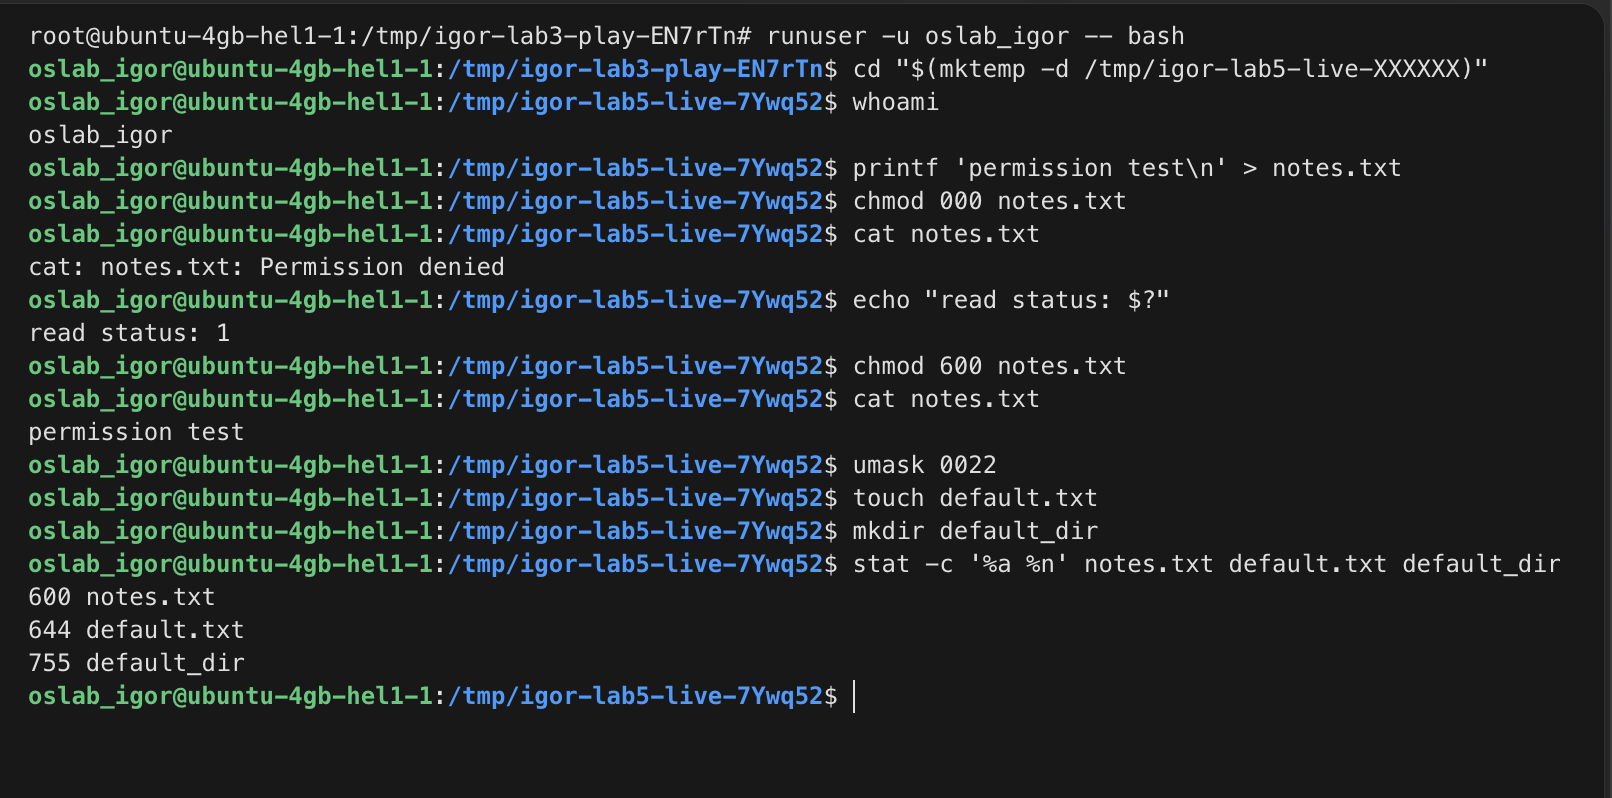
\includegraphics[width=\linewidth,height=0.67\textheight,keepaspectratio]{Lab5-6/evidence/screenshots/lab5-permissions-terminal.png}
\end{minipage}\par\medskip

\subsection{Scope and implementation}\label{scope-and-implementation}

This experiment examines two different tasks: reading metadata for a
supplied name and walking a directory tree to discover names. The
complete implementations are included as
{\ttfamily\fontsize{10}{12}\selectfont xv6/user/mys\allowbreak{}tat.c}
and
{\ttfamily\fontsize{10}{12}\selectfont xv6/user/fin\allowbreak{}d.c},
together with their UPROGS entries and the full kernel tree needed to
build them. The following results were collected from that tree in QEMU
with one emulated hart, using a fresh generated filesystem image.

The required README/r2 sequence was run first, including removing README
and reading r2. README was then restored through a hard link so later
trace tests could use it. An additional disposable file named specimen
checks the behavior on a short payload. The test tree contains both file
and directory matches.

\subsection{Part 1 Types and empty
directories}\label{part-1-types-and-empty-directories}

Types 1, 2 and 3 mean directory, regular file and device. Root has inode
1; dot and dot-dot both identify it because root is its own parent. A
new directory a occupied 32 bytes, representing two 16-byte directory
entries: a two-byte inode number and fourteen-byte name, for dot and
dot-dot. The public stat structure exposes dev, ino, type, nlink and
size.

\par\noindent\begin{minipage}{\linewidth}

\begin{lstlisting}
$ mkdir a
$ ls a
.              1 35 32
..             1 1 1024
\end{lstlisting}

\end{minipage}\par

\subsection{Reading metadata without confusing a name with an
inode}\label{reading-metadata-without-confusing-a-name-with-an-inode}

{\ttfamily\fontsize{10}{12}\selectfont mystat} loops over its operands
and calls {\ttfamily\fontsize{10}{12}\selectfont stat} for each one. It
translates the three public xv6 types into file, directory, and device
labels, and prints the inode number, link count, and byte size. If one
lookup fails, it records failure and continues through later operands
instead of aborting at the first bad name. The size uses the format for
a 64-bit unsigned value rather than treating the field as a small
integer.

README initially reported inode 2, one link and 2441 bytes. After ln,
README and r2 shared inode 2 and two links. After removing README, r2
retained inode 2 and size 2441 with one link, and cat could still read
its contents. The extra ten-byte specimen received inode 40 in this
image and showed the same link behavior.

\par\noindent\begin{minipage}{\linewidth}

\begin{lstlisting}
$ mystat README . console
README: type=file inode=2 links=1 bytes=2441
.: type=directory inode=1 links=4 bytes=1024
console: type=device inode=30 links=1 bytes=0
$ ln README r2
$ mystat README r2
README: type=file inode=2 links=2 bytes=2441
r2: type=file inode=2 links=2 bytes=2441
$ rm README
$ mystat r2
r2: type=file inode=2 links=1 bytes=2441
$ cat r2 | wc
48 336 2441
\end{lstlisting}

\end{minipage}\par

\par\noindent\begin{minipage}{\linewidth}

\begin{lstlisting}
$ echo igor-file > specimen
$ mystat specimen
specimen: type=file inode=40 links=1 bytes=10
$ ln specimen alias
$ mystat specimen alias
specimen: type=file inode=40 links=2 bytes=10
alias: type=file inode=40 links=2 bytes=10
$ rm specimen
$ mystat alias
alias: type=file inode=40 links=1 bytes=10
$ cat alias
igor-file
$ mystat missing-path
mystat: cannot stat missing-path
\end{lstlisting}

\end{minipage}\par

Inode numbers depend on allocation order. The tested invariant is that
both names identify one inode and that removing one name preserves the
remaining link and contents.

\subsection{Part 3 Measuring the
limits}\label{part-3-measuring-the-limits}

BSIZE is 1024, NDIRECT is 12, NINDIRECT is 1024 divided by a four-byte
block number, and DIRSIZ is 14. Maximum file payload is
{\ttfamily\fontsize{10}{12}\selectfont (12 + 1024/4) * 1024 = 274432}
bytes, or 268 KiB. The indirect block is metadata, not part of that
payload.

Creating averyveryverylongname stored the fourteen-character name
averyveryveryl. The builder reported 2000 blocks: 47 metadata and 1953
data. Metadata comprises two boot/super blocks, 31 log blocks including
its header, 13 inode blocks and one bitmap block.

\par\noindent\begin{minipage}{\linewidth}

\begin{lstlisting}
42:#define IPB (BSIZE / sizeof(struct dinode))
5:#define BSIZE   1024 // block size
26:#define NDIRECT   12
27:#define NINDIRECT (BSIZE / sizeof(uint))
54:#define DIRSIZ 14
nmeta 47 (boot, super, log blocks 31, inode blocks 13, bitmap blocks 1) blocks 1953 total 2000
$ mkdir averyveryverylongname
$ ls
averyveryveryl 1 36 32
[Other listing entries are retained in the full recording.]
\end{lstlisting}

\end{minipage}\par

The on-disk dinode fields are type, major, minor, nlink, size and twelve
direct addresses plus one indirect address. A name is stored in a
directory entry, not in the inode. Major and minor identify a device for
a device inode.

\subsection{Part 4 A find implementation that also reports
directories}\label{part-4-a-find-implementation-that-also-reports-directories}

The search utility takes a starting pathname and a basename. After stat
it compares the current name before deciding whether to recurse,
allowing directories themselves to match. It copies the fixed-width
{\ttfamily\fontsize{10}{12}\selectfont dirent.name} into a
DIRSIZ-plus-one buffer and adds a terminator rather than assuming the
kernel entry is already a C string.

The loop skips unused entries, dot, and dot-dot. Before constructing a
child path, it checks the parent, separator, name, and terminator
against its 512-byte buffer. Lookup and read failures produce
diagnostics and a failure status. Every opened directory is closed after
traversal. Ancestor descriptors remain open during recursion, so very
deep trees are limited by xv6's descriptor limit.

\subsection{Tests that distinguish traversal from correct
matching}\label{tests-that-distinguish-traversal-from-correct-matching}

The tree contains {\ttfamily\fontsize{10}{12}\selectfont tree/target}
and
{\ttfamily\fontsize{10}{12}\selectfont tree/branch/\allowbreak{}target},
plus a directory
{\ttfamily\fontsize{10}{12}\selectfont tree/branch/\allowbreak{}targetdir}.
Searching for {\ttfamily\fontsize{10}{12}\selectfont target} printed the
two files; searching for
{\ttfamily\fontsize{10}{12}\selectfont targetdir} printed the directory;
searching for {\ttfamily\fontsize{10}{12}\selectfont branch} printed the
intermediate directory. A fourteen-character filename checked the DIRSIZ
boundary, and a missing starting path exercised the diagnostic path.
Invoking {\ttfamily\fontsize{10}{12}\selectfont find} without the two
operands printed usage rather than interpreting uninitialized arguments.

\par\noindent\begin{minipage}{\linewidth}

\begin{lstlisting}
$ mkdir tree
$ mkdir tree/branch
$ echo root-copy > tree/target
$ echo nested-copy > tree/branch/target
$ mkdir tree/branch/targetdir
$ find tree target
tree/branch/target
tree/target
$ find tree targetdir
tree/branch/targetdir
$ find tree branch
tree/branch
$ echo edge > tree/abcdefghijklmn
$ find tree abcdefghijklmn
tree/abcdefghijklmn
$ find missing-path target
find: cannot stat missing-path
$ find
usage: find start basename
$
\end{lstlisting}

\end{minipage}\par

These tests would expose a common bug in which basename comparison is
performed only for regular files. Such a version can descend into
{\ttfamily\fontsize{10}{12}\selectfont branch} and still fail to print
{\ttfamily\fontsize{10}{12}\selectfont branch} or
{\ttfamily\fontsize{10}{12}\selectfont targetdir}. The directory-target
assertions in
{\ttfamily\fontsize{10}{12}\selectfont scripts/run-\allowbreak{}xv6.py}
verify that behavior explicitly. The raw console output is retained in
{\ttfamily\fontsize{10}{12}\selectfont Lab5-6/evide\allowbreak{}nce/xv6.txt},
so the displayed paths can be checked against the commands that
constructed them.

\subsection{Why unlink does not always free the blocks
immediately}\label{why-unlink-does-not-always-free-the-blocks-immediately}

In
{\ttfamily\fontsize{10}{12}\selectfont kernel/sysfi\allowbreak{}le.c},
the {\ttfamily\fontsize{10}{12}\selectfont ip->nlink--;} line in
{\ttfamily\fontsize{10}{12}\selectfont sys\_unlink} decrements the link
count after removing the name. In
{\ttfamily\fontsize{10}{12}\selectfont kernel/fs.c},
{\ttfamily\fontsize{10}{12}\selectfont iput} waits for zero links and
the final relevant in-memory reference before
{\ttfamily\fontsize{10}{12}\selectfont itrunc} frees data blocks. An
open reference can therefore preserve an unlinked inode.

The experiment proves survival through another hard link. The
open-but-unlinked explanation comes from source inspection; it is a
separate lifetime case.

Running
{\ttfamily\fontsize{10}{12}\selectfont scripts/run-\allowbreak{}xv6.py}
rebuilds the image and checks these distinctive link and search results.
A fresh generated disk prevents leftover test names from affecting a
rerun.

\subsection{Execution captures and code
excerpts}\label{execution-captures-and-code-excerpts}

The following native Terminal screenshots were supplied by the author
from direct source inspection and live xv6 execution. They replace the
saved-record browser views. This additional run uses l6live\_note and
l6live\_link (inode 48, 10 bytes, link counts 1 then 2 then 1), and a
separate l6live directory tree. Earlier measurements in the report refer
to the original specimen and tree fixtures retained in the raw
transcript; inode numbers and directory link counts depend on filesystem
state.

\par

\medskip\noindent

\begin{minipage}{\linewidth}\setstretch{1.0}
\captionof*{figure}{Figura 2. Native xv6 execution: metadata and hard links}
\centering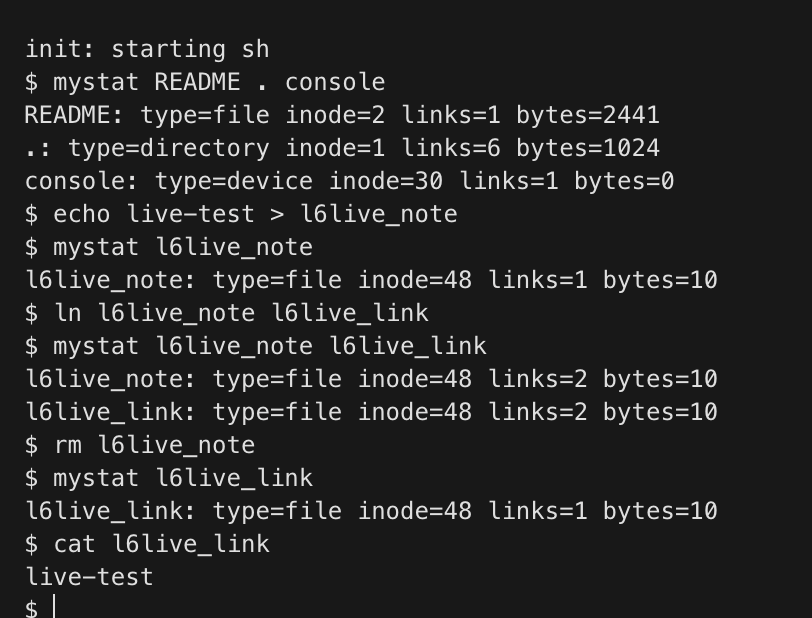
\includegraphics[width=\linewidth,height=0.67\textheight,keepaspectratio]{Lab5-6/evidence/screenshots/lab6-mystat-execution-terminal.png}
\end{minipage}\par\medskip

\par

\medskip\noindent

\begin{minipage}{\linewidth}\setstretch{1.0}
\captionof*{figure}{Figura 3. Native xv6 execution: recursive basename search and error paths}
\centering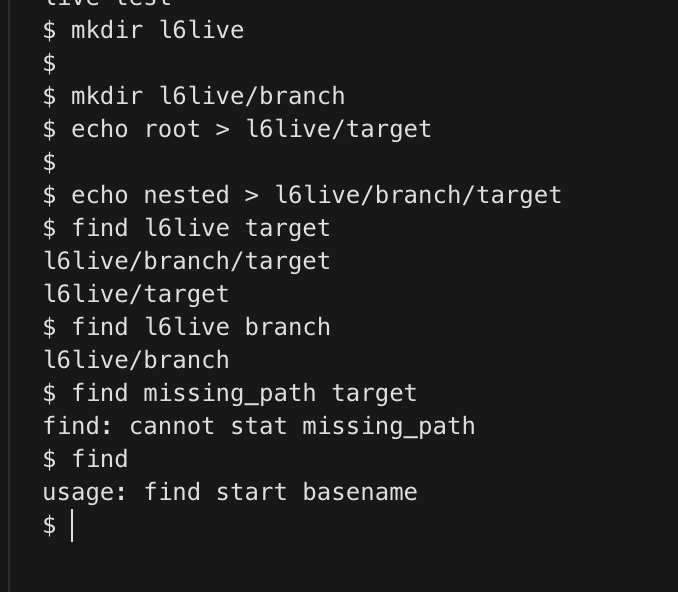
\includegraphics[width=\linewidth,height=0.67\textheight,keepaspectratio]{Lab5-6/evidence/screenshots/lab6-find-execution-terminal.png}
\end{minipage}\par\medskip

\par

\medskip\noindent

\begin{minipage}{\linewidth}\setstretch{1.0}
\captionof*{figure}{Figura 4. Native Terminal: mystat source and Makefile registration}
\centering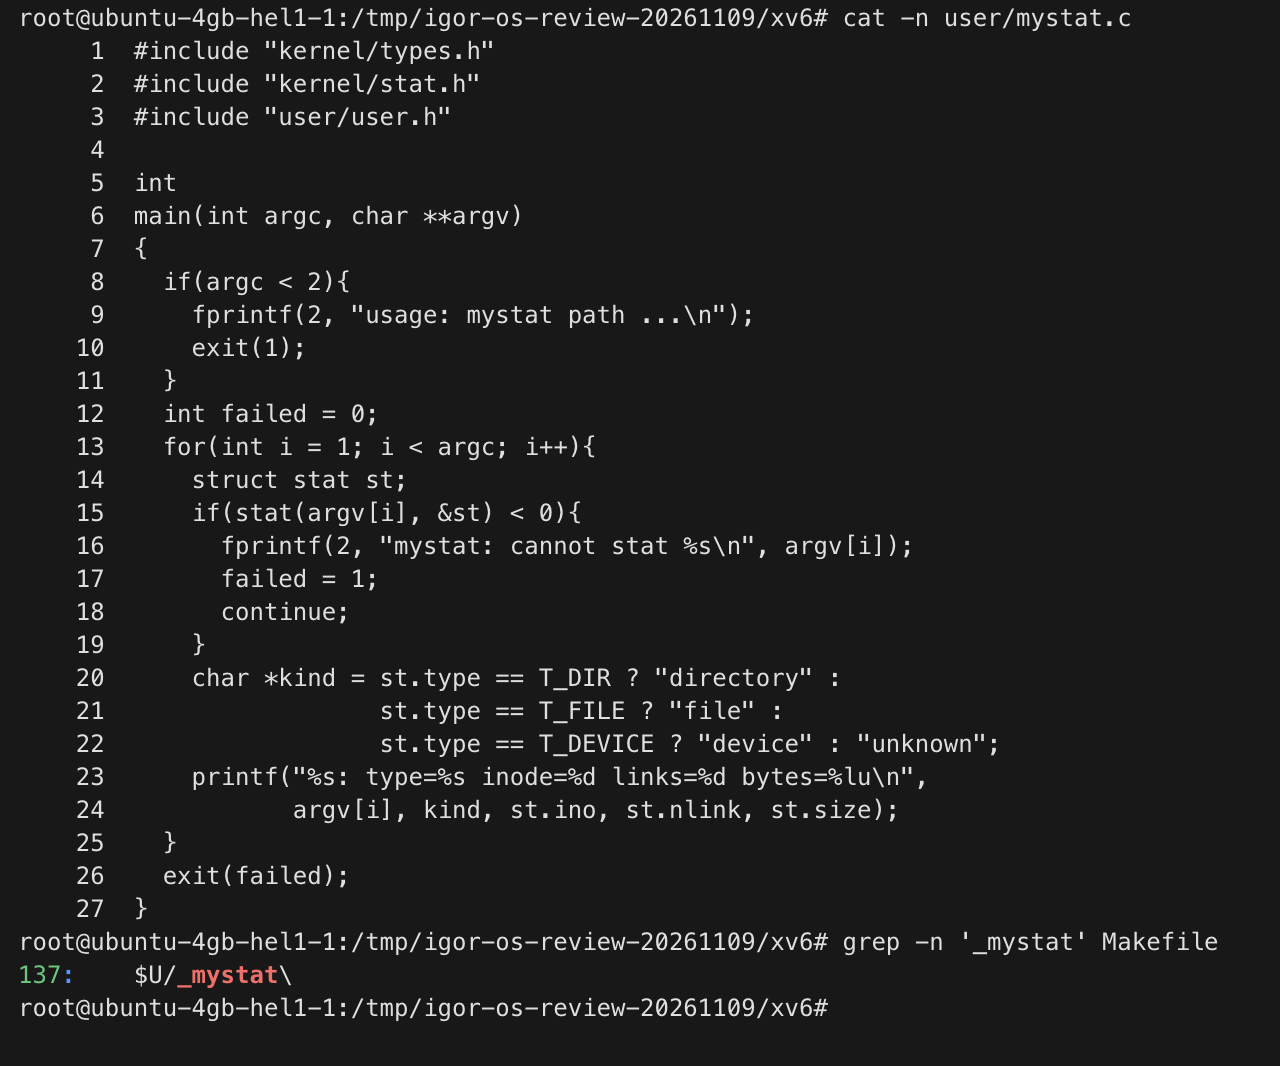
\includegraphics[width=\linewidth,height=0.67\textheight,keepaspectratio]{Lab5-6/evidence/screenshots/lab6-mystat-source-terminal.png}
\end{minipage}\par\medskip

\par

\medskip\noindent

\begin{minipage}{\linewidth}\setstretch{1.0}
\captionof*{figure}{Figura 5. Native Terminal: find recursive traversal source and Makefile registration}
\centering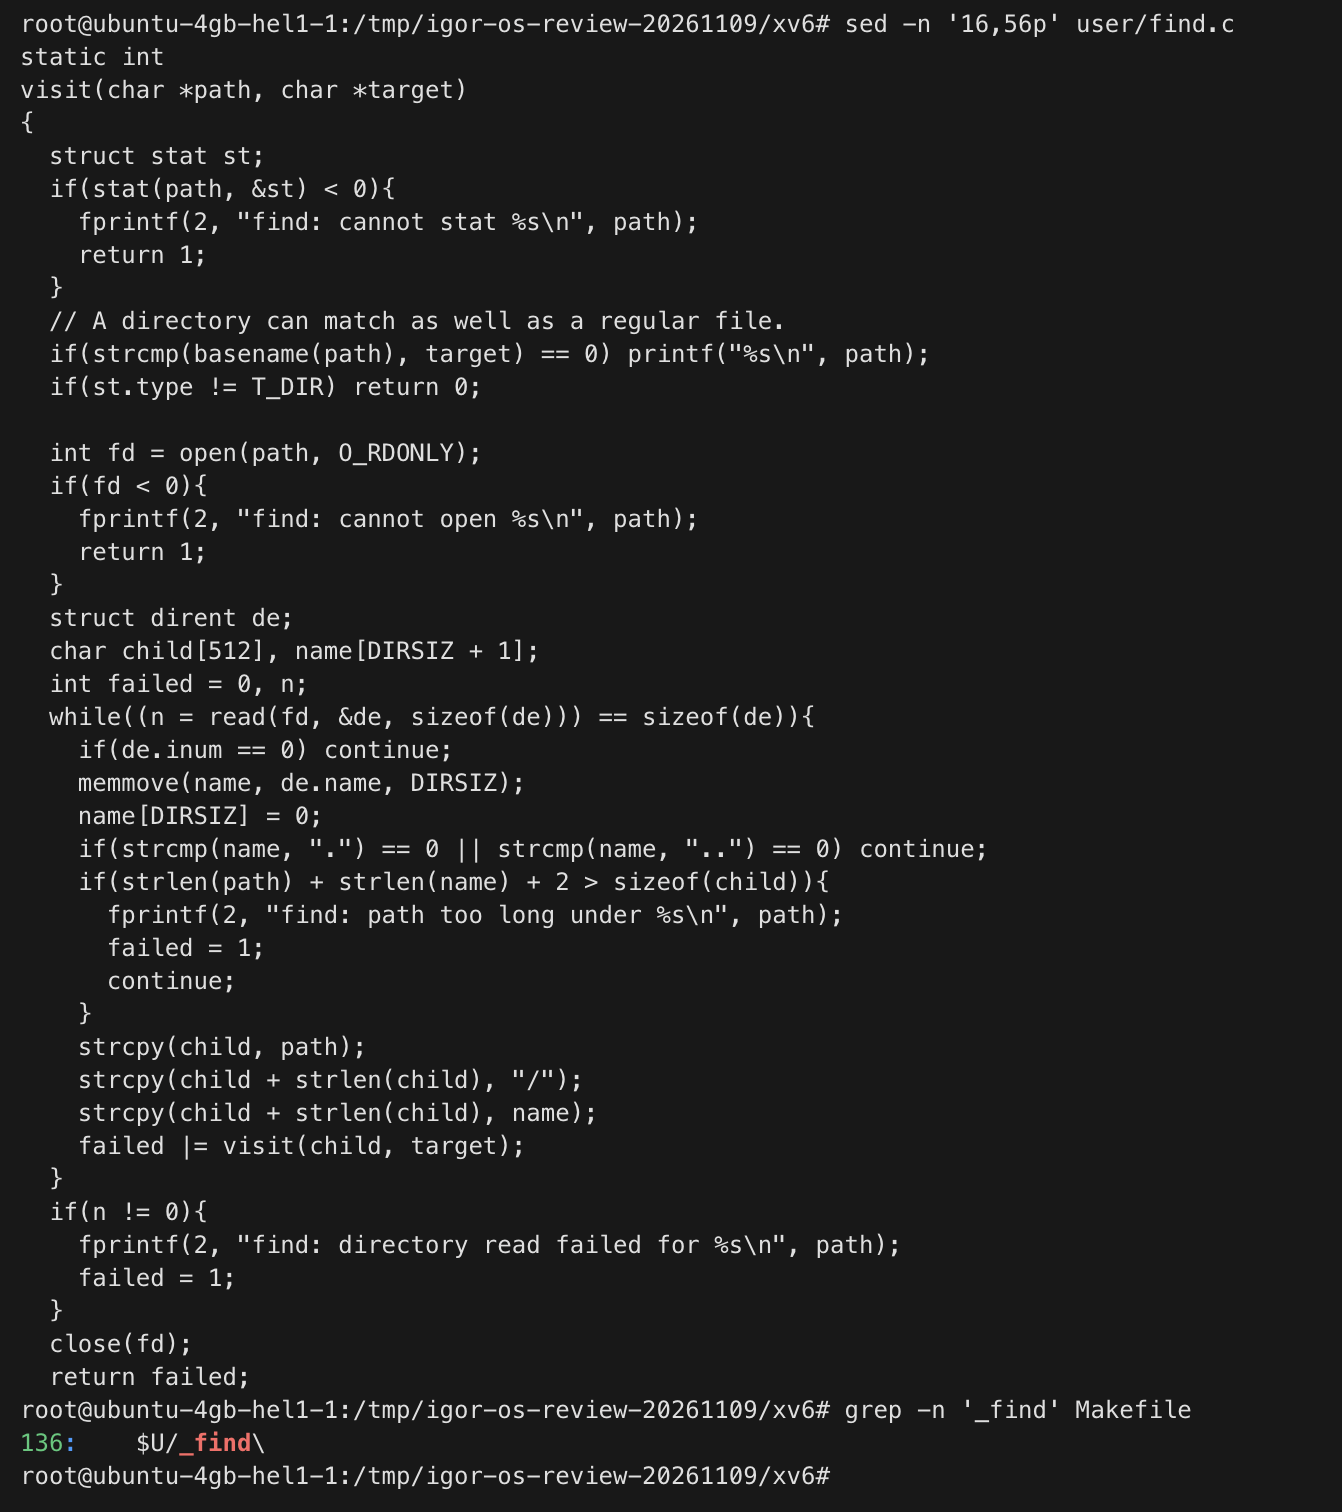
\includegraphics[width=\linewidth,height=0.67\textheight,keepaspectratio]{Lab5-6/evidence/screenshots/lab6-find-source-terminal.png}
\end{minipage}\par\medskip

\par\noindent\begin{minipage}{\linewidth}

\section{Concluzie}\label{concluzie}

Testele separă numele, inode-ul și datele fișierului și arată efectul
legăturilor și al permisiunilor. Utilitarele xv6 reproduc aceste
observații prin apeluri de sistem, cu rezultate și erori verificabile în
surse și capturi.

\end{minipage}\par

\end{document}
